\documentclass[UTF8,12pt]{ctexart}
\usepackage[a4paper,margin=1.5cm]{geometry}
\usepackage{graphicx}
\usepackage{float}
\usepackage{caption}
\setlength{\parindent}{0pt}
\captionsetup{font=small,labelformat=empty}
\begin{document}
\section*{高一数学专题题目归档：立体几何}
来源：\verb|documents/高一|，按 OCR 关键词筛选后裁剪原题图。共 9 题。

\subsection*{1. 原卷第 3 题}
\textbf{来源}：【期末】上海市复旦大学附属中学2024-2025学年第二学期高一数学期末试卷（B）

\begin{figure}[H]
\centering
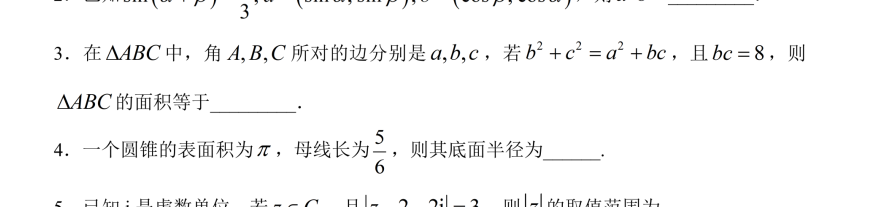
\includegraphics[width=0.96\linewidth]{crops/07-lXolUr-1bu6QRhI1-002-q03.png}
\caption{原图：\detokenize{documents/高一/07-lXolUr-1bu6QRhI1/002.png}}
\end{figure}
\vspace{0.4em}
\subsection*{2. 原卷第 7 题}
\textbf{来源}：【期末】上海市复旦大学附属中学2024-2025学年第二学期高一数学期末试卷（B）

\begin{figure}[H]
\centering
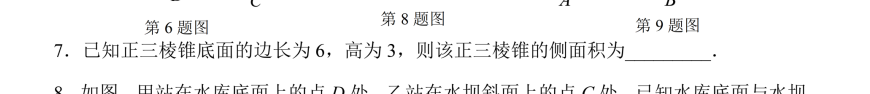
\includegraphics[width=0.96\linewidth]{crops/07-lXolUr-1bu6QRhI1-002-q07.png}
\caption{原图：\detokenize{documents/高一/07-lXolUr-1bu6QRhI1/002.png}}
\end{figure}
\vspace{0.4em}
\subsection*{3. 原卷第 8 题}
\textbf{来源}：【期末】上海市复旦大学附属中学2024-2025学年第二学期高一数学期末试卷（B）

\begin{figure}[H]
\centering
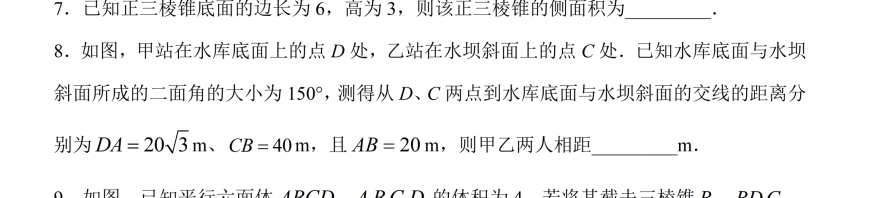
\includegraphics[width=0.96\linewidth]{crops/07-lXolUr-1bu6QRhI1-002-q08.png}
\caption{原图：\detokenize{documents/高一/07-lXolUr-1bu6QRhI1/002.png}}
\end{figure}
\vspace{0.4em}
\subsection*{4. 原卷第 9 题}
\textbf{来源}：【期末】上海市复旦大学附属中学2024-2025学年第二学期高一数学期末试卷（B）

\begin{figure}[H]
\centering
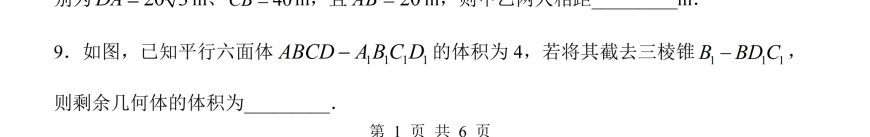
\includegraphics[width=0.96\linewidth]{crops/07-lXolUr-1bu6QRhI1-002-q09.png}
\caption{原图：\detokenize{documents/高一/07-lXolUr-1bu6QRhI1/002.png}}
\end{figure}
\vspace{0.4em}
\subsection*{5. 原卷第 12 题}
\textbf{来源}：【期末】上海市复旦大学附属中学2024-2025学年第二学期高一数学期末试卷（B）

\begin{figure}[H]
\centering
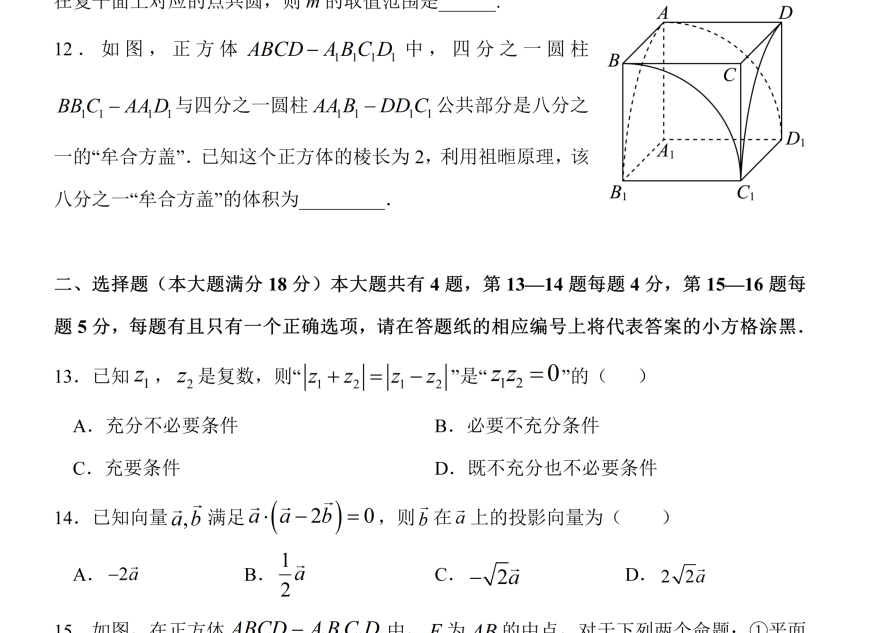
\includegraphics[width=0.96\linewidth]{crops/07-lXolUr-1bu6QRhI1-003-q12.png}
\caption{原图：\detokenize{documents/高一/07-lXolUr-1bu6QRhI1/003.png}}
\end{figure}
\vspace{0.4em}
\subsection*{6. 原卷第 15 题}
\textbf{来源}：【期末】上海市复旦大学附属中学2024-2025学年第二学期高一数学期末试卷（B）

\begin{figure}[H]
\centering
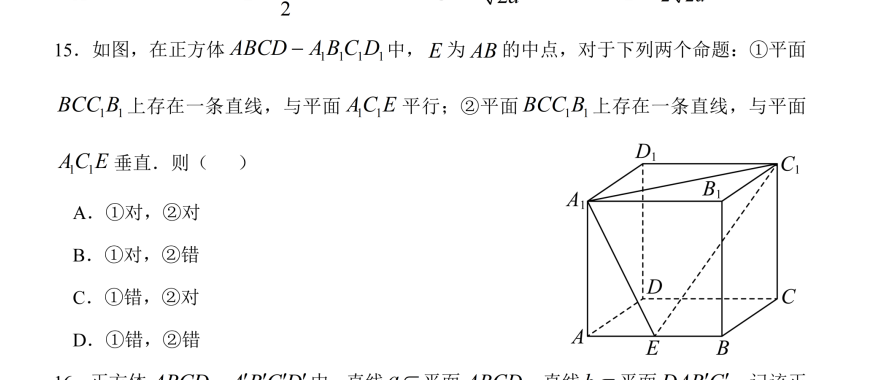
\includegraphics[width=0.96\linewidth]{crops/07-lXolUr-1bu6QRhI1-003-q15.png}
\caption{原图：\detokenize{documents/高一/07-lXolUr-1bu6QRhI1/003.png}}
\end{figure}
\vspace{0.4em}
\subsection*{7. 原卷第 16 题}
\textbf{来源}：【期末】上海市复旦大学附属中学2024-2025学年第二学期高一数学期末试卷（B）

\begin{figure}[H]
\centering
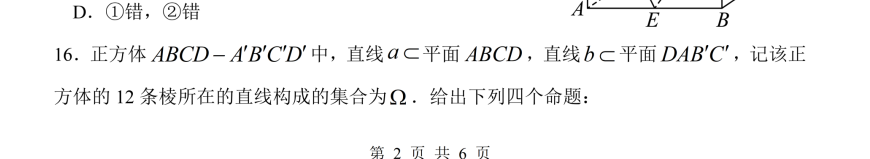
\includegraphics[width=0.96\linewidth]{crops/07-lXolUr-1bu6QRhI1-003-q16.png}
\caption{原图：\detokenize{documents/高一/07-lXolUr-1bu6QRhI1/003.png}}
\end{figure}
\vspace{0.4em}
\subsection*{8. 原卷第 18 题}
\textbf{来源}：【期末】上海市复旦大学附属中学2024-2025学年第二学期高一数学期末试卷（B）

\begin{figure}[H]
\centering
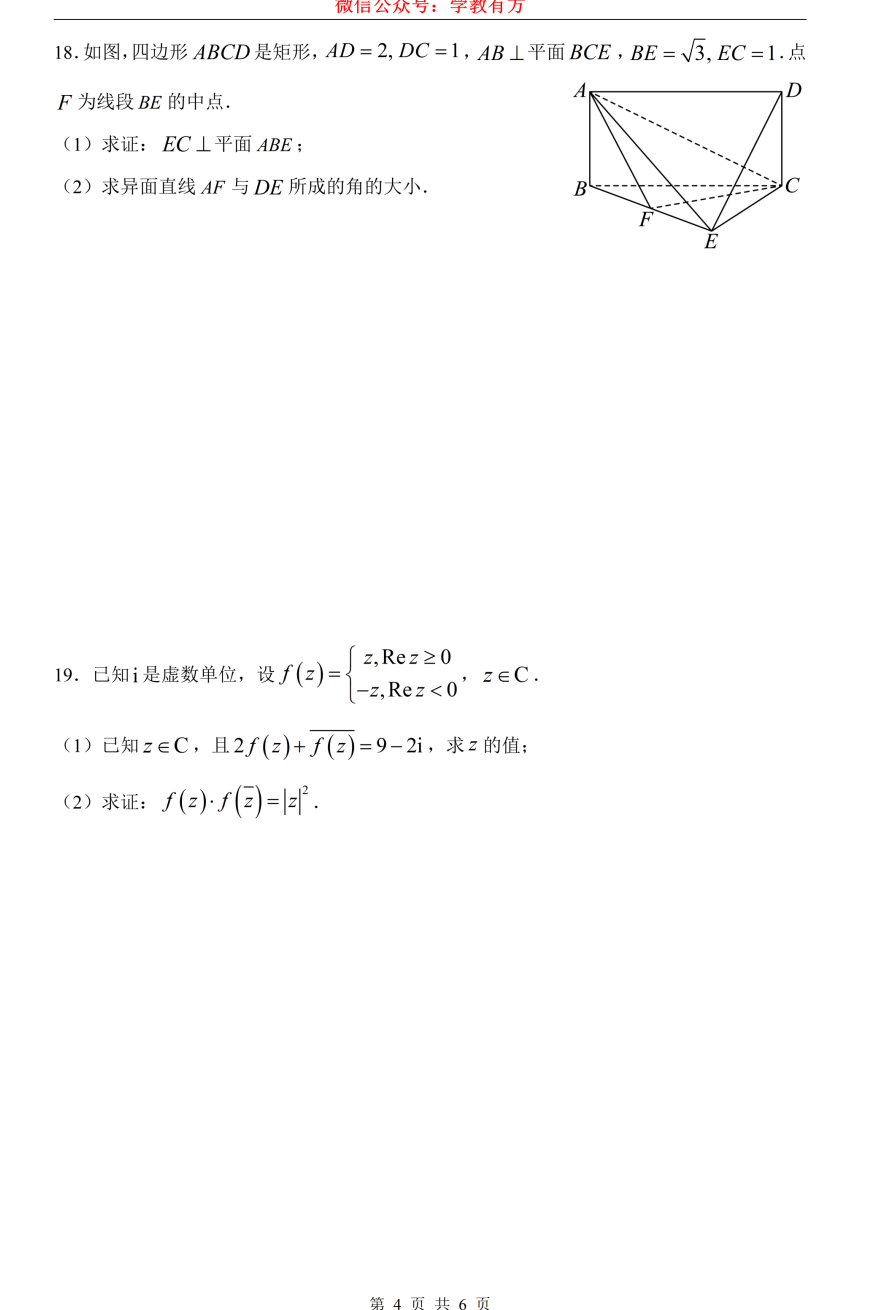
\includegraphics[width=0.96\linewidth]{crops/07-lXolUr-1bu6QRhI1-005-q18.png}
\caption{原图：\detokenize{documents/高一/07-lXolUr-1bu6QRhI1/005.png}}
\end{figure}
\vspace{0.4em}
\subsection*{9. 原卷第 20 题}
\textbf{来源}：【期末】上海市复旦大学附属中学2024-2025学年第二学期高一数学期末试卷（B）

\begin{figure}[H]
\centering
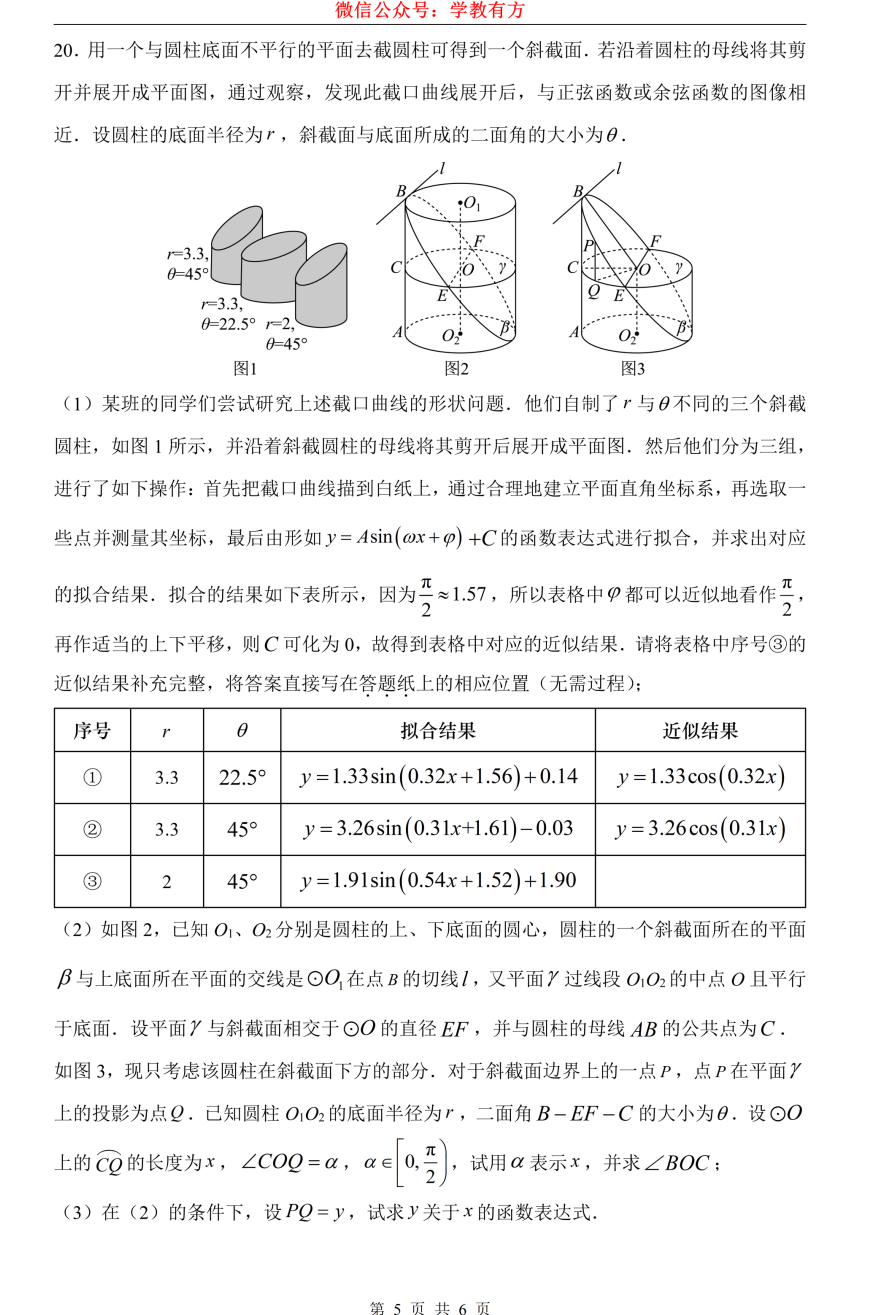
\includegraphics[width=0.96\linewidth]{crops/07-lXolUr-1bu6QRhI1-006-q20.png}
\caption{原图：\detokenize{documents/高一/07-lXolUr-1bu6QRhI1/006.png}}
\end{figure}
\vspace{0.4em}
\end{document}
